\documentclass[11pt]{article}
\usepackage[margin=2.54cm]{geometry}
\usepackage{amsfonts, amsmath, amssymb}
\usepackage{graphicx}
\graphicspath{ {images/} }
\usepackage{hyperref}
\setlength{\parindent}{0em}

\begin{document}
\section{Problem definition}
\setcounter{page}{1}
KPMG's report on "The alcoholic beverages market in Poland" claims, that in 2013, Poles spent 41.1 billion zlotys on alcohol, with beer being a large portion of that amount (47\%) \cite{kpmg_alco}. The report also states that, as of 2014, Polish customers choose beers based on premiumisation (31\% of customers), innovation (29\%) and region affiliations (30\%), with manufacturers predicting significant rise of interest in those attributes in the future \cite{kpmg_alco}. The evolution in customers' taste and their openness resulted in many local shops offering a vast range of, so called, "craft beers" coming from lesser known breweries. However, it's also not uncommon to stumble upon large product shelves, with dozens different beers types, in more popular Polish stores like Lidl and Carrefour.\\

\begin{figure}[h]
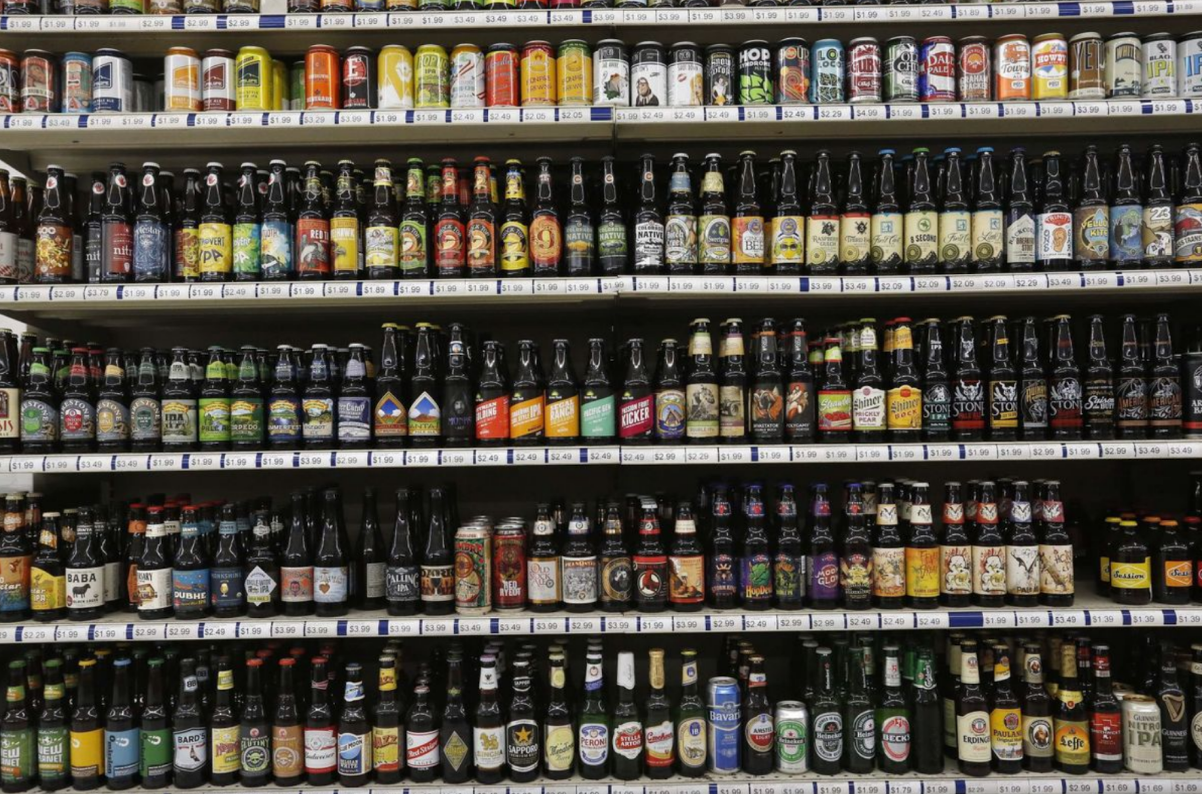
\includegraphics[width=0.5\textwidth]{beer_shelf}
\centering
\caption{A large beer shelf. Source: \protect \url{http://trib.com}.}.
\label{fig:beer_shelf}
\end{figure}

The question this thesis posed at first was "How technology could be used to help a customer, who stands in front of a supermarket's large beer shelf (\autoref{fig:beer_shelf}.) and tries to choose one, not knowing anything about beers?". The answer appeared to be relatively simple and involved developing a mobile application, which could connect to beer database residing in Cloud e. g. Firebase Realtime Database and retrieve details about any given beer. The real problem, that later emerged, and is in fact the basis of this thesis, is "Given a mobile application, that can connect to beer database in Cloud, what is the most intuitive, appealing and fastest way of accessing this database from the device?".
\clearpage

\section{Solution overview}

\clearpage
\bibliography{mybib}
\bibliographystyle{siam}
\end{document}